\documentclass[10pt, conference, compsocconf,letter]{IEEEtran}   	
%\usepackage{geometry}                		% See geometry.pdf to learn the layout options. There are lots.
%\geometry{letterpaper}                		% ... or a4paper or a5paper or ... 
%\geometry{landscape}                		% Activate for for rotated page geometry
%\usepackage[parfill]{parskip}    		% Activate to begin paragraphs with an empty line rather than an indent
\usepackage{graphicx}				% Use pdf, png, jpg, or eps§ with pdflatex; use eps in DVI mode
						% TeX will automatically convert eps --> pdf in pdflatex

\usepackage{color}
\newcommand{\fix}[1]{\textcolor{red}{#1}}
\newcommand{\highlight}[1]{\textcolor{red}{#1}}
\usepackage{amssymb, amsmath}
\usepackage{mathtools}
\usepackage{booktabs}
%\usepackage[noend]{algpseudocode}
%\usepackage[ruled,vlined]{algorithm2e}
\usepackage{verbatim}
\newcommand*\rot{\rotatebox{90}}
%\usepackage[compatible]{algpseudocode}
\usepackage{algorithm}
\usepackage[noend]{algpseudocode}
\usepackage{varwidth}
\usepackage{multirow}
\usepackage{rotating, xcolor}
\usepackage{subfig}
\usepackage{enumitem}
%\usepackage[caption=false]{subfig}
\usepackage[hyphens]{url}
\usepackage{float}
\newfloat{algorithm}{t}{lop}

\usepackage{tcolorbox}
\definecolor{mycolor}{rgb}{0.122, 0.435, 0.698}
%\begin{tcolorbox}[width=\linewidth, boxsep=0pt, left=-4pt, boxrule=0.5pt]
%\end{tcolorbox} 
%\newtcolorbox{mybox}{colback=red!5!white,colframe=mycolor}
\makeatletter
\newcommand{\mybox}[1]{%
  %\setbox0=\hbox{#1}%
  %\setlength{\@tempdima}{\dimexpr\wd0+13pt}%
  \begin{tcolorbox}[colframe=mycolor,boxrule=0.5pt,arc=4pt,
      left=-4pt,right=6pt,top=6pt,bottom=6pt,boxsep=0pt,width=\linewidth]
    #1
  \end{tcolorbox}
}
\makeatother

\algnewcommand{\LineComment}[1]{\State \(\triangleright\) #1}
%\newcommand{\procdecl}[1]   {\proc{#1}\vrule width0pt height0pt depth 7pt \relax}
\newcommand{\lilabel}[1]        {\label{li:#1}}

\newcommand{\erdosrenyi}{Erd\H os-R\'{e}nyi }
\newcommand{\qg}{\u{g}}
\newcommand{\qG}{\u{G}}
\newcommand{\qc}{\c{c}}
\newcommand{\qC}{\c{C}}
\newcommand{\qs}{\c{s}}
\newcommand{\qS}{\c{S}}
\newcommand{\qu}{\"{u}}
\newcommand{\qU}{\"{U}}
\newcommand{\qo}{\"{o}}
\newcommand{\qO}{\"{O}}
\newcommand{\qI}{\.{I}}
\newcommand{\wa}{\^{a}}
\newcommand{\wA}{\^{A}}
\usepackage{mathtools}
\DeclarePairedDelimiter\ceil{\lceil}{\rceil}
\DeclarePairedDelimiter\floor{\lfloor}{\rfloor}


\newcommand{\minusone}{\text{-}1}

%% ABAB: Shortcuts/macros below are not used but it can be referenced as a cheatsheet
\newcommand{\liref}[1]      {line~\ref{li:#1}}
\newcommand{\Liref}[1]      {Line~\ref{li:#1}}
\newcommand{\lirefs}[2]     {lines \ref{li:#1}--\ref{li:#2}}
\newcommand{\Lirefs}[2]     {Lines \ref{li:#1}--\ref{li:#2}}
\newcommand{\lireftwo}[2]   {lines \ref{li:#1} and~\ref{li:#2}}
\newcommand{\lirefthree}[3] {lines \ref{li:#1}, \ref{li:#2}, and~\ref{li:#3}}

\def\Cpp{C{}\texttt{++}}
\newcommand{\mA}{\mathbf{A}} 
\newcommand{\mL}{\mathbf{L}}
\newcommand{\mU}{\mathbf{U}}
\newcommand{\transpose}     {^{\mbox{\scriptsize \sf T}}}
\newcommand{\mB}{\mathbf{B}}
\newcommand{\mC}{\mathbf{C}}
\newcommand{\dimN}{n}
\newcommand{\dimM}{m}
\newcommand{\dimK}{k}
\newcommand{\dnzc}{\id{nzc}}
\newcommand{\dnzr}{\id{nzr}}
\newcommand{\dni}{\id{ni}}
\newcommand{\dnnz}{\id{nnz}}
\newcommand{\dsort}{\id{sort}}
\newcommand{\dscan}{\id{scan}}
\newcommand{\dsearch}{\id{search}}
\newcommand{\dmin}{\func{min}}
\newcommand{\dmax}{\func{max}}
\newcommand{\dth}{th}
\newcommand{\dlen}{\id{len}}
\newcommand{\matlab}{{\sc Matlab}}

%
%TGM: included and new commands from our graphBLAS C API document
%
\usepackage{listings}
\renewcommand{\vector}[1]{{\bf #1}}
\renewcommand{\matrix}[1]{{\bf #1}}
\renewcommand{\arg}[1]{{\sf #1}}
\newcommand{\zip}{{\mbox{zip}}}
\newcommand{\zap}{{\mbox{zap}}}
\newcommand{\ewiseadd}{{\mbox{\bf ewiseadd}}}
\newcommand{\ewisemult}{{\mbox{\bf ewisemult}}}
\newcommand{\mxm}{{\mbox{\bf mxm}}}
\newcommand{\vxm}{{\mbox{\bf vxm}}}
\newcommand{\mxv}{{\mbox{\bf mxv}}}
\newcommand{\gpit}[1]{{\sf #1}}
\newcommand{\ie}{\emph{i.e.}}
\newcommand{\eg}{\emph{e.g.}}
\newcommand{\nan}{{\sf NaN}}
\newcommand{\nil}{{\bf nil}}
\newcommand{\ifif}{{\bf if}}
\newcommand{\ifthen}{{\bf then}}
\newcommand{\ifelse}{{\bf else}}
\newcommand{\ifendif}{{\bf endif}}
\newcommand{\zero}{{\bf 0}}
\newcommand{\one}{{\bf 1}}
\newcommand{\true}{{\sf true}}
\newcommand{\false}{{\sf false}}
\newcommand{\syntax}{{C Syntax}}
%%%%%%

%\input{algobox}

\title{Design of the GraphBLAS API for C}

\author{
Ayd\i n Bulu\qc , Tim Mattson, Scott McMillan, Jos\'e Moreira, Carl Yang}

\date{}	

\begin{document}
\maketitle

\begin{abstract}

The purpose of the GraphBLAS Forum is to standardize linear-algebra
building blocks for graph computations.  An important part of this
standardization effort is to translate the mathematical specification
into an actual Application Programming Interface (API) that (i) is
faithful to the mathematics and (ii) enables efficient implementations
on modern hardware. This paper documents the approach taken by the C
language specification subcommittee and presents the main concepts,
constructs, and objects within the GraphBLAS API.

\end{abstract}

%%%%%%%%%%%%%%%%%%%%%%% file intro.tex %%%%%%%%%%%%%%%%%%%%%%%%%
%
% This file contains the introduction section of the paper
%
%%%%%%%%%%%%%%%%%%%%%%%%%%%%%%%%%%%%%%%%%%%%%%%%%%%%%%%%%%%%%%%%%%%
\section{Introduction}
\label{sec:intro}
The GraphBLAS are great and you'll love them.  In this paper, we'll talk about the even greater stuff coming in the future
\section{GraphBLAS Math}
\label{sec:math}

Consider a graph represented in terms of an adjacency matrix and a second
matrix representing a subset of the vertices in the graph.  The traditional
matrix product over real arithmetic of these two matrices returns the
cost based on the accumulated edge weights of reaching the 
set of vertices connected to the initial vertices.   This fundamental
operation can be used to construct a wide range of graph algorithms.

We can extend the range of graph operations by keeping the basic
pattern of a matrix-matrix multiplication, but varying
the operators and the interpretation of the values in the matrices (the \emph{domain}).
By carefully choosing operators and the domain, we control the
relation between matrix operations familiar in linear algebra and graph operations, thereby enabling
composable graph algorithms.

This generalized matrix multiplication is performed on an algebraic semiring.   A semiring is an algebraic
structure over a domain $D$ with two binary operations $\oplus$ and $\otimes$.
The \emph{addition} operator, $\oplus$, is a commutative monoid with an identity element $\bold{0}$ (not necessarily the number 0)
while the \emph{multiplication} operator, $\otimes$, is a commutative monoid with an 
identity element $\bold{1}$ (not necessarily the number 1).  The additive identity is also an annhilator for the multiplication 
operator ($\otimes$) and multiplication distributes with addition.  The most 
common semirings used in the Graph Algorithms community are 
shown in table~\ref{Tab:semirings}.
  
\begin{table}[h]
\hrule
\begin{center}
\caption{Common semirings used with graph algorithms.}
\label{Tab:semirings}
\begin{tabular}{llllll}
{\sf Semiring} 			& \multicolumn{2}{c}{operators} & domain 					& $\bold{0}$ 	& $\bold{1}$ \\
				& $\oplus$	& $\otimes$	& \\	
\hline
Standard arithmetic        	& $ + $ 	& $ \times $  	& $\mathbb{R}$					& $0$		& $1$ \\
max-plus algebras           	& $ \max $ 	& $ + $  	& $\{-\infty \cup  \mathbb{R} \}$		& $-\infty$ & $0$ \\
max-min algebras           	& $ \max $ 	& $ \times $  	& $\infty \cup  \mathbb{R}_{\leq 0}$\\
Galois fields (\eg, GF2)     	& $ \xor $	& $ \mbox{and} $& $\{0, 1\}$					& $0$           & $1$ \\
Power set algebras         	& $ \cup $ 	& $ \cap $  	& $\mathbb{Z}$\\
\end{tabular}
\end{center}
\hrule
\end{table}

It is often convenient to change the semiring applied
to a given matrix.  This means we must represent the matrix and the semiring separately and disassociated in GraphBLAS,
and the two come together only when an operation is performed.
Mathematically, the ability to change semirings 
when moving from one GraphBLAS operation with a matrix to the next impacts the meaning of 
the \emph{implied zero} in a sparse representation of the matrix.
This element in real arithmetic is the number zero ($0$), which is the 
identity of the addition operator and the annihilator of
multiplication operator.   As the semiring changes, this 
implied or \emph{structural zero} changes to the identity of 
the addition operator and the annihilator of the multiplication 
operator for the new semiring.   Nothing changes in the
stored matrix, but the implied values within the sparse matrix change
with respect to a particular operation.  

This feature has significant impact on the definitions of the operations in the GraphBLAS.   
Consider matrix multiplication over the domain $\mathbb{S}$ 
with semiring operators 
$\oplus$ and $\otimes$:
 $$
   \mathbf{C} = \mathbf{A} {\oplus}.{\otimes} \mathbf{B} = \mathbf{A} \mathbf{B}.
$$
Using index notation familiar in linear algebra
  $$
   {\bf C}(i,j) = \bigoplus_{k=1}^l {\bf A}(i,k) \otimes {\bf B}(k,j)
  $$
for matrices with dimensions
$$
  {\bf A} : \mathbb{S}^{m \times l} ~~~~~
  {\bf B} : \mathbb{S}^{l \times m} ~~~~~
  {\bf C} : \mathbb{S}^{m \times n}
$$
The summation notation only works, however, if we redefine the implied zero of the 
sparse matrices as we change the semiring (to the corresponding additive identity).   Depending on the domains associated with the
matrix elements and the operations, this can lead to awkward definitions of the
operations involving the structural zeros.  A cleaner approach based on set notation
avoids this problem.  For example, we can define the previous matrix multiplication
as:   
$$
\bold{C}(i,j)
= \bigoplus_{k \in \bold{ind}(\matrix{{A}}(i,:)) \cap
\bold{ind}(\matrix{{B}}(:,j))} (\matrix{{A}}(i,k)
\otimes \matrix{{B}}(k,j)),
$$ 
where $\bold{ind}(\matrix{{A}}(i,:))$ is the set of the column indices of the 
nonzero elements of row $i$ of matrix $\bold{A}$, and
$\bold{ind}(\matrix{{B}}(:,j))$ is the set of the row indices of the 
nonzero elements of column $j$ of matrix $\bold{B}$.

In other words, the binary operation $\otimes$ is applied to the elements in the intersection of the 
two sets $\bold{ind}(\matrix{{A}}(i,:))$ and $\bold{ind}(\matrix{{B}}(:,j))$, and the results of which are accumulated using the $\oplus$ operator.
These notations are equivalent but by defining the pairwise operations over
the set intersections, we never have to define how the additive identity defined by one
semiring interacts with the structural zeros defined by a different semiring.

In addition to matrix multiplication, the GraphBLAS math specification defines
a range of additional operations.  These are summarized in table~\ref{Tab:GraphBLASOps}.
In addition to matrices, these operations also manipulate \emph{vectors}, which are
one-dimensional structures (as opposed to the two-dimensions matrices).

\begin{table}[h]
\hrule
\begin{center}
\caption{A Mathematical overview of the fundamental GraphBLAS operations supported
in this specification. $\matrix{A}$, $\matrix{B}$, and $\matrix{C}$ are GraphBLAS matrices; 
$\vector{u}$, $\vector{v}$, and $\vector{w}$ are GraphBLAS vectors; $i$ and $j$ are single indices;
$\bold{i}$ and $\bold{j}$ are arrays of indices;
$\bold{val}$ is an array of element values;  $f()$ is a function.
While not shown here, the input 
matrices $\matrix{A}$ and $\matrix{B}$ may be selected for transposition prior to 
the operation and masks can be used to control which values are written to the output GraphBLAS object.}
\label{Tab:GraphBLASOps}
\begin{tabular}{l|rrl}
{\sf Operation name} & \multicolumn{3}{c}{Mathematical description}  \\
\hline
{\sf mxm}          & $\matrix{C}$ & $\oplus=$ & $\matrix{A} \oplus.\otimes \matrix{B}$  \\
{\sf mxv}          & $\vector{v}$ & $\oplus=$ & $\matrix{A} \oplus.\otimes \vector{u}$  \\
{\sf vxm}          & $\vector{v}$ & $\oplus=$ & $\vector{u} \oplus.\otimes \matrix{A}$  \\
{\sf eWiseMult}    & \multicolumn{3}{c}{$\matrix{C} = \matrix{C} \oplus (\matrix{A} \otimes \matrix{B}) ; \vector{w} = \vector{w} \oplus (\vector{u} \otimes \vector{v})$} \\
{\sf eWiseAdd}     & \multicolumn{3}{c}{$\matrix{C} = \matrix{C} \oplus (\matrix{A} \oplus \matrix{B}) ; \vector{w} = \vector{w} \oplus (\vector{u} \oplus \vector{v})$} \\
{\sf reduce} (row) & $\vector{u}$ & $\oplus=$ & $\oplus_j\matrix{A}(:,j)$  \\
{\sf apply}        & $\matrix{C}$ & $\oplus=$ & $f(\matrix{A})$ \\
{\sf transpose}    & $\matrix{C}$ & $\oplus=$ & $\matrix{A}^T$ \\
{\sf extract}      & $\matrix{C}$ & $\oplus=$ & $\matrix{A}(\vector{i},\vector{j})$ \\
{\sf assign}       & $\matrix{C}(\vector{i},\vector{j})$ & $\oplus=$ & $\matrix{A}$ \\
%{\sf buildMatrix}  & $\matrix{C}$ & $\oplus=$ & $\mathbb{S}^{m\times n}(\vector{i},\vector{j},\vector{v},\oplus_{dup})$ \\
%{\sf buildVector}  & $\vector{u}$ & $\oplus=$ & $\mathbb{S}^{n}(\vector{i},\vector{v})$ \\
{\sf extractTuples}& $(\vector{i},\vector{j},\vector{val})$ & $=$ & $\matrix{A}$ \\
\end{tabular}
\end{center}
\hrule
\end{table}


\section{GraphBLAS objects}
\label{sec:GrBObjects}

The GraphBLAS C API is built on objects exposed to 
the C programmer as opaque data types. These objects include
\begin{itemize}
\item \emph{Collections}: vectors and matrices.
\item \emph{Algebraic objects}: unary and binary operators, monoids, and semirings.
\item \emph{Control objects}: descriptors and masks (both one- and two-dimensional).
\end{itemize}

Functions that manipulate GraphBLAS objects
are referred to as {\it methods}.  These methods fully define the 
interface to create or destroy GraphBLAS objects, modify their 
contents, and copy the contents of opaque objects into non-opaque or \emph{transparent} 
objects, the contents of which are under direct observation and control of the programmer

\subsection{Collections}
\label{Sec:Collections}

The state of a GraphBLAS application is largely captured by collections of values, 
namely vectors and matrices.  The GraphBLAS collections 
are opaque objects only accessible through the methods in the GraphBLAS C API.
The use of opaque data types gives the implementation the flexibility needed to 
aggressively optimize for different system architectures.

A GraphBLAS vector $\vector{v} = \langle D, N, \{ (i,v_i) \} \rangle$ is defined by:
\begin{itemize}
\item The domain $D$, which is the data type for the elements of the vector.
\item The size $N>0$.
\item A set of tuples $(i,v_i)$ where $0 \leq
i < N$ and $v_i \in D$. 
\end{itemize}
A particular value of $i$ can only appear at
most once in $\vector{v}$. We define $\mathbf{nelem}(\vector{v}) = N$ and
$\mathbf{L}(\vector{v}) = \{ (i,v_i) \}$. The set $\mathbf{L}(\vector{v})$ is
called the \emph{content} of vector $\vector{v}$. 
%%%%
% TGM:  Any concepts we don't use in the paper should not be introduced, 
% hence why these are commented out
%%%%
%We also define the set:
%$$
%\vector{ind(\vector{v})} = \{ i : (i,v_i) \in \mathbf{L}(\vector{v}) \}
%$$
%(called the \emph{structure} of $\vector{v}$), and $\mathbf{D}(\vector{v})
%= D$. 
For a vector $\vector{v}$, $\vector{v}(i)$ is a reference to $v_i$
if $(i,v_i) \in \mathbf{L}(\vector{v})$ and is undefined otherwise. 

A GraphBLAS matrix  $\matrix{A} = \langle D, M, N, \{ (i,j,A_{ij}) \} \rangle$ is
defined by:
\begin{itemize}
\item The domain $D$, which is the data type for the elements of the matrix.
\item The number of rows $M>0$ and columns $N>0$.
\item A set of tuples $\mathbf{L}(\matrix{A}) = (i,j,A_{ij})$ where $0 \leq i < M$, $0 \leq
j < N$, and $A_{ij} \in D$. 
\end{itemize}
A particular pair of values $i,j$ can only
appear at most once in $\matrix{A}$. 
The set $\mathbf{L}(\matrix{A})$ is called the
\emph{content} of matrix $\matrix{A}$.  
We also define $\mathbf{nrows}(\matrix{A}) = M$ and 
$\mathbf{ncols}(\matrix{A}) = N$.
%%%%%
% TGM: if we don't use a notation in this paper, then I don't want to introduce it
%%%%%
%We define $\mathbf{ncols}(\matrix{A})
%= N$,  $\mathbf{nrows}(\matrix{A}) = M$ and $\mathbf{L}(\matrix{A}) =
%\{ (i,j,A_{ij}) \}$.  
%We also define the sets:
%$$
%\vector{indrow(\matrix{A})} = \{ i : \exists (i,j,A_{ij}) \in \matrix{A} \}
%$$
%$$
%\vector{indcol(\matrix{A})} = \{ j : \exists(i,j,A_{ij}) \in \matrix{A} \}
%$$  
%These are the sets of nonempty
%rows and columns of $\matrix{A}$, respectively.)  The \emph{structure}
%of matrix $\matrix{A}$ is the set 
%$$
%\mathbf{ind}(\matrix{A}) = \{ (i,j) :(i,j,A_{ij}) \in \mathbf{L}(\matrix{A}) \}
%$$
%and $\mathbf{D}(\matrix{A}) = D$.
For a matrix $\matrix{A}$, $\matrix{A}(i,j)$ is a reference to $A_{ij}$
if $(i,j,A_{ij}) \in \mathbf{L}(\matrix{A})$ and is undefined otherwise.  

The fact that matrix and vector elements can be undefined is an essential difference between GraphBLAS
and more traditional sparse matrix packages for which elements that are not
explicitly stored are assumed to have the numerical value $0$.   We leave these
elements as undefined to avoid the complexity of interpreting these implied
values differently as the operation semiring changes.

If $\matrix{A}$ is a matrix and $0 \leq j < N$, then 
$$ \matrix{A}(:,j)= \langle D, M, \{(i,A_{ij}) : (i,j,A_{ij}) \in \mathbf{L}(\matrix{A})\} \rangle
$$
is a vector called the $j$-th \emph{column}
of $\matrix{A}$. Correspondingly, if $\matrix{A}$ is a matrix and
$0 \leq i < M$, then 
$$
\matrix{A}(i,:) = \langle D, N, \{(j,A_{ij}) :(i,j,A_{ij}) \in \mathbf{L}(\matrix{A}) \} \rangle
$$ 
is a vector called
the $i$-th \emph{row} of $\matrix{A}$.

We define the transpose of a matrix in the traditional manner where
row and column indices are swapped.   Consider a matrix 
$
\matrix{A} = \langle D, M, N, \{ (i,j,A_{ij}) \} \rangle,
$
the \emph{transpose} of $\matrix{A}$ is the matrix 
$$
\matrix{A}^T = \langle D, N, M, \{(j,i,A_{ij}) : (i,j,A_{ij}) \in \mathbf{L}(\matrix{A}) \} \rangle.
$$

\subsection{Algebraic objects}
\label{Sec:AlgebraicObjects}

The GraphBLAS differs from traditional sparse linear algebra APIs in that the
algebra associated with the data can be varied to match the needs
of an application.  Pragmatically, this means the API was designed to
provide a great deal of flexibility in the domains of the elements in the GraphBLAS
collections and the operations defined between these elements.

We start with  basic binary and unary operators.  
A GraphBLAS \emph{binary operator} is defined as:
$$
F_b = \langle D_1, D_2, D_3, \odot \rangle.
$$
It has three domains, $D_1$, $D_2$, $D_3$, and an operation
$$
\odot: D_1 \times D_2 \rightarrow D_3.
$$
%For a given GraphBLAS operators
%$$
%F_b=\langle D_1, D_2, D_3,\odot \rangle
%$$ we define $\mathbf{D}_1(F_b) = D_1$,
%$\mathbf{D}_2(F_b) = D_2$, $\mathbf{D}_3(F_b) = D_3$, and $\mathbf{\bigodot}(F_b)
%= \odot$.  Note that $\odot$ could be used in place of either $\oplus$ or $\otimes$.
A GraphBLAS \emph{unary operators} is defined as:
$$
F_u = \langle D_1, D_2, f\rangle.
$$
It has two domains, $D_1$, $D_2$, and an operation
$f: D_1 \rightarrow D_2$.  
%For a given GraphBLAS operators
%$$
%F_u=\langle D_1, D_2, f \rangle
%$$ we define $\mathbf{D}_1(F_u) = D_1$,
%$\mathbf{D}_2(F_u) = D_2$, and $\mathbf{f}(F)
%= f$.
%

GraphBLAS makes use of two fundamental algebraic structures: monoids
and semirings.   
A GraphBLAS  \emph{monoid} 
$$
M =\langle D_1,\odot,\mathbf{0} \rangle
$$ 
is defined by a single domain $D_1$, an 
\emph{associative}\footnote{It is expected that implementations 
will utilize IEEE-754 floating point arithmetic which is not 
strictly associative.} 
operation $\odot: D_1 \times D_1 \rightarrow D_1$,
and an identity element $\mathbf{0} \in D_1$.  
%For a given GraphBLAS monoid
%$$
%M=\langle D_1,\odot,0 \rangle
%$$ 
%we define $\mathbf{D}_1(M) = D_1$, $\mathbf{\bigodot}(M) =
%\odot$ and $\mathbf{0}(M) = 0$.  
Let
$
F = \langle D_1,D_1,D_1,\odot \rangle
$ 
be a GraphBLAS binary operator and let
$\mathbf{0}$ be the identity for $\odot$. Then 
$$
M = \langle F,\mathbf{0} \rangle = \langle
D_1,\odot,\mathbf{0} \rangle
$$ 
is the associated GraphBLAS monoid.

The algebraic structure at the core of the GraphBLAS is the semiring.  
A GraphBLAS \emph{semiring} 
$$
S=\langle D_1,D_2,D_3,\oplus,\otimes,\mathbf{0} \rangle
$$ 
is defined by
three domains $D_1$, $D_2$ and $D_3$, an \emph{associative}
additive operation 
$$
\oplus : D_3 \times D_3 \rightarrow D_3
$$
a multiplicative operation 
$$\otimes : D_1 \times D_2 \rightarrow
D_3
$$
and an element $\mathbf{0} \in D_3$, which is the identity for $\oplus$.
%For a given GraphBLAS semiring 
%$$
%S=\langle D_1,
%D_2, D_3,\oplus,\otimes,0 \rangle
%$$ 
%we define $\mathbf{D}_1(S) = D_1$,
%$\mathbf{D}_2(S) = D_2$, $\mathbf{D}_3(S) = D_3$, $\mathbf{\bigoplus}(S) =
%\oplus$, $\mathbf{\bigotimes}(S) = \otimes$, and $\zero(S) = 0$. 

Let $F = \langle D_1,D_2,D_3,\otimes \rangle$ be a GraphBLAS binary operator
and let $M = \langle D_3,\oplus,\mathbf{0} \rangle$ be a GraphBLAS monoid,
then 
$$
S= \langle M,F \rangle = \langle D_1,D_2,D_3,\oplus,\otimes,\mathbf{0} \rangle
$$
is a GraphBLAS semiring.

Correspondingly, for a GraphBLAS semiring 
$S = \langle D_1,D_2,D_3,\oplus,\otimes,\mathbf{0} \rangle$
there is always an associated monoid 
$M = \langle D_3,\oplus,\mathbf{0} \rangle$ and
an associated binary operator $F = \langle D_1,D_2,D_3,\otimes \rangle$.

A UML diagram of the conceptual hierarchy of Algebraic objects in GraphBLAS
algebra (binary operators, monoids and semirings) is shown in 
Figure~\ref{Fig:AlgebraHierarchy}.

\begin{figure}[htb]
    \hrule
    \begin{center}
        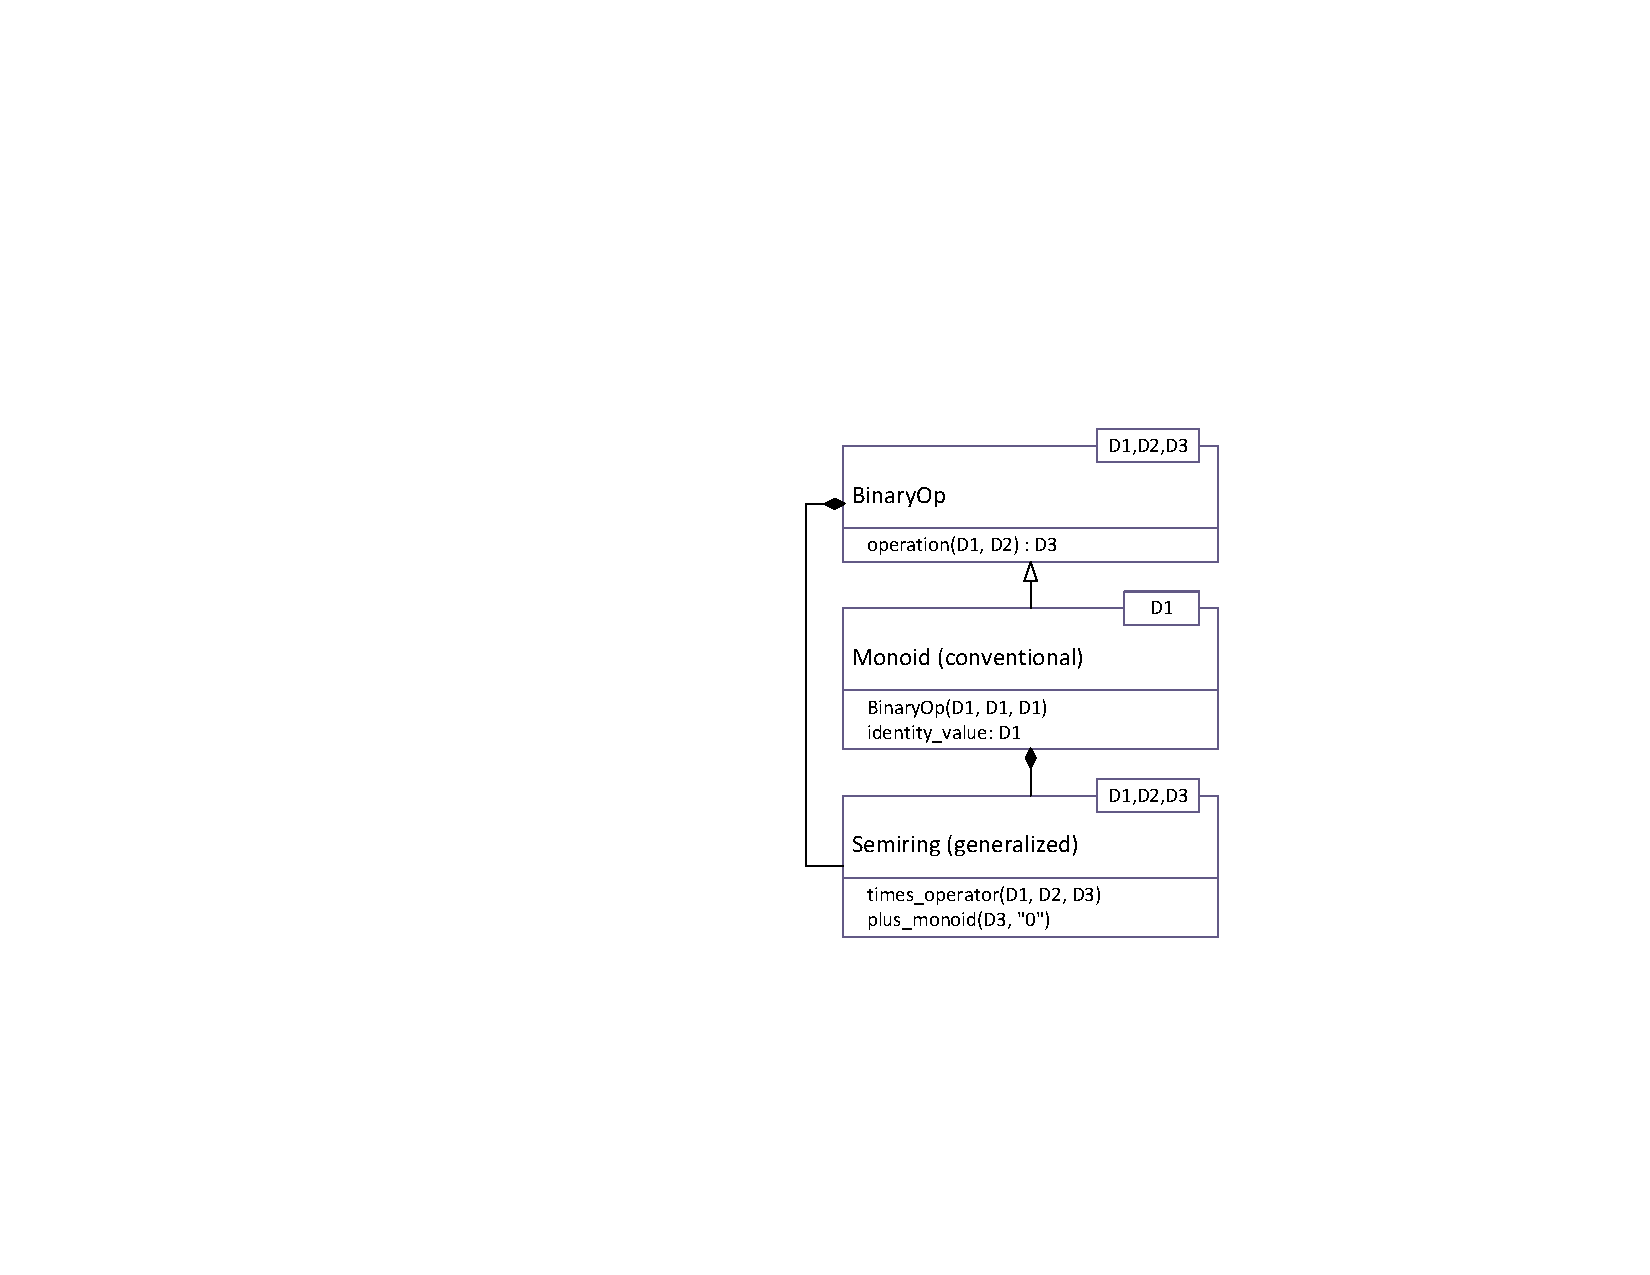
\includegraphics[width=1.0\linewidth,trim=3in 2in 0.5in 2in]{Algebra_Hierarchy_v2.pdf}
    \end{center}
    \caption{Hierarchy of algebraic object classes in GraphBLAS. GraphBLAS semirings consist of a conventional monoid with one domain for the addition function, and a binary operator with three domains for the multiplication function.}
    \label{Fig:AlgebraHierarchy}
    \hrule
\end{figure}


\subsection{Control objects}
\label{Sec:ControlObjects}

The GraphBLAS C API specification defines two opaque objects that 
modify the semantics of GraphBLAS methods; \emph{masks} and 
\emph{descriptors}.  

A mask can be either a one- or a two-dimensional construct.  One- and
two-dimensional masks, described more formally below, are similar to
vectors and matrices, respectively, except that they have structure
(indices) but no values. Masks are used to control which values from 
a operation are written to the output object.

A one-dimensional mask $\vector{m} = \langle N, \{ i \} \rangle$ is
defined by its number of elements $N>0$ and a set $\mathbf{L}(\vector{m})$
of indices $\{ i \}$ where $0 \leq i < N$.  A particular value of $i$ can
only appear at most once in $\vector{m}$. We define $\mathbf{nelem}(\vector{m})
= N$.  
We define the \emph{structure} of a one dimensional mask as the set
$\mathbf{L}(\vector{m})$.
%% JEM: For masks, L(m) and ind(m) are identical. Let us see if we can avoid defining ind(m).
%% $$
%% \vector{ind(\vector{m})} = \{ i : i \in
%% \mathbf{L}(\vector{m}) \}
%% $$

A two-dimensional mask
$
\matrix{M} = \langle M, N, \{ (i,j) \}
\rangle
$
is defined by its number of rows $M>0$, its number of
columns $N>0$ and a set $\mathbf{L}(\matrix{M})$ of tuples $(i,j)$
where $0 \leq i < M$, $0 \leq j < N$.   A particular pair of values
$i,j$ can only appear at most once in $\matrix{M}$.  
%We define
%$\mathbf{ncols}(\matrix{M}) = N$, and $\mathbf{nrows}(\matrix{M}) = M$.
The \emph{structure} of a two-dimensional mask $\matrix{M}$ is the set
$\mathbf{L}(\matrix{M})$.
We also define $\mathbf{nrows}(\matrix{M}) = M$ and
$\mathbf{ncols}(\matrix{M}) = N$.
%% $$
%% \mathbf{ind}(\matrix{M}) = \{ (i,j) : (i,j) \in \mathbf{L}(\matrix{M}) \}
%% $$

Operations may be directed to use the \emph{structural complement} of a mask.
For a one-dimensional mask $\vector{m}$ this is denoted as
$\neg\vector{m}$. For a two-dimensional mask $\matrix{M}$ this is denoted as
$\neg\matrix{M}$.  The structure of the complement of an one-dimensional
mask $\vector{m}$ is defined as:
$$
\mathbf{L}(\neg\vector{m}) = \{i : 0
\leq i < N, i \notin \mathbf{L}(\vector{m}) \}
$$
It is the set of all
possible indices that do not appear in $\vector{m}$.  The structure
of the complement of a two-dimensional mask $\matrix{M}$ is defined as:
$$
\mathbf{L}(\neg\matrix{M}) = \{(i,j) : 0 \leq i < M, 0 \leq j < N,
(i,j) \notin \mathbf{L}(\matrix{M}) \}
$$
It is the set of all possible indices that do not appear in $\matrix{M}$.

The second control object is the \emph{descriptor}.  Descriptors
modify the semantics of GraphBLAS methods by controlling additional optional behaviors. 
In particular, descriptors specify how other input arguments 
-- vectors, matrices and masks -- should be processed (modified) 
before the main operation of a method is performed.  It is
also used to specify whether the output argument should be cleared before assignment.

The descriptor is a lightweight object.  It pairs a set of flags
representing the possible modifiers with each mask, vector or matrix argument of a
GraphBLAS method.  For example, a descriptor may specify that a particular 
input matrix needs to be transposed or that a mask needs to be structurally 
complemented before using it in the operation.

For the purpose of constructing descriptors, the arguments of a method
that can be modified are identified by specific field names. The output parameter (typically
the first parameter in a GraphBLAS method) is indicated by the field name, 
{\sf GrB\_OUTP}.  The mask is indicated by the {\sf GrB\_MASK} field name. The input parameters
corresponding to the input vectors and matrices are indicated by {\sf GrB\_INP0},
{\sf GrB\_INP1}, and so on, in the order they appear in the signature of the GraphBLAS method.

\section{GraphBLAS Execution Model}
\label{sec:GrBExec}

A program using the GraphBLAS C API constructs GraphBLAS objects,
manipulates them to implement a graph algorithm, and then extracts values 
from the GraphBLAS objects as the result of the algorithm.  Functions defined
within the GraphBLAS C API that manipulate GraphBLAS objects are called
\emph{methods}.

Graph algorithms are expressed as an ordered collection of GraphBLAS method calls
defined by the order they are encountered in a program.  This is called the 
\emph{Program Order}.  Each method in the collection uniquely and unambiguously
defines the output GraphBLAS objects based on the GraphBLAS operation and the input 
GraphBLAS objects.

We define a sequence of GraphBLAS method calls, or when the meaning is clear a \emph{sequence},
as a well defined ordered collection of GraphBLAS method calls.  The begining of a sequence
is the first method call that modifies a GraphBLAS object, after the end of the previous sequence (if any).  The end of the sequence is either (1) the first 
GraphBLAS method that reads values from a GraphBLAS object into a non-opaque data structure
or (2) a GraphBLAS wait method.  We collectively refer to these methods as \emph{terminating methods}.
The set of operations between the initiation of a sequence and its termination mathematically define the result of that sequence. 

A GraphBLAS program executes in one of two modes: \emph{blocking} and \emph{nonblocking}.  
\begin{itemize}
\item \emph{blocking}: In blocking mode, each method in a sequence completes the GraphBLAS operation 
defined by the method before proceeding to the next statement in program order.  Output GraphBLAS
objects defined by a method are stored in memory and are available to other C functions after each
method returns.

\item \emph{nonblocking}: In nonblocking mode, each method may return once the input arguments have 
been inspected and verified to define a well formed GraphBLAS operation.  The GraphBLAS operation
and the state of any GraphBLAS objects are undefined when a method returns until the 
terminating method in the sequence returns.
\end{itemize}

An application executing in nonblocking mode is not required to return immediately after input arguments have 
been verified. In essence, a conforming implementation of the GraphBLAS C API running in 
nonblocking mode may choose to execute ``as if'' in blocking mode.   
Further, a sequence in nonblocking mode where
every GraphBLAS operation is followed by a call to a GraphBLAS wait method
is equivalent to the same sequence in blocking mode with GraphBLAS wait methods  removed. 

Nonblocking mode allows for any execution strategy that 
satisfies the mathematical definition of the sequence.  The methods can be placed into
a queue and deferred.  They can be chained together and fused (\eg,
replacing a chained pair of matrix products with a matrix triple product).
Lazy evaluation, greedy evaluation or asynchronous execution are all
valid as long as the final result agrees with the mathematical 
definition provided by the sequence of GraphBLAS method calls
appearing in  program order.

Blocking mode forces an implementation to carry out precisely the GraphBLAS operations
defined by the methods and to store output objects to memory between method calls.  
It is valuable for debugging or in cases where an external tool needs to 
evaluate the state of memory during a sequence.

In a  mathematically well-defined sequence with input objects that are well-conditioned, the results
from blocking and nonblocking modes should be identical outside of effects due to round-off errors 
associated with floating point arithmetic.   Due to the great flexibility afforded to 
an implementation when using nonblocking mode, we expect execution of a 
sequence in nonblocking mode to potentially complete execution in less time.

The mode is defined in the GraphBLAS C API when the context of the library invocation 
is defined.  This occurs once before any GraphBLAS methods are called with a call to the
{\sf GrB\_init()} function.   After all GraphBLAS methods are complete, the context is terminated
with a call to {\sf GrB\_finalize()}.  In the current version of the GraphBLAS C API, the context can only be 
set once in the execution of a program. That is, after {\sf GrB\_finalize()} is called a following call to
{\sf GrB\_init()} is not allowed.

\section{Error Model}
\label{sec:GrBError}

All GraphBLAS methods return a value of type {\sf GrB\_info} to provide
information available to the system at the time the method returns.�
In blocking mode, that information pertains to the full computation and
the return values defined for each method in the specification provide
information concerning the condition of the computation.�

In nonblocking mode, the information pertains to a consistency check
of the arguments to the method. Any method that terminates a sequence
must return information about the status of that sequence of method
calls.� A return value of {\sf GrB\_SUCCESS} indicates that the method
returned correctly and that the sequence produced the result defined
by the sequence of GraphBLAS operations.�� Other return values from
the method indicate that an error was found during execution of the
sequence.� When possible, that return value will provide information
concerning the cause of the error.� Additional information is returned
in the null terminated character string, {\sf err} which is always the
last argument to any method that may terminate a sequence.�

Errors fall into two groups: API errors and execution errors.  An API error
means a GraphBLAS method was called with parameters that violate the
rules for that method. API errors are deterministic and consistent across
platforms and implementations.  Execution errors indicate that something
went wrong during the execution of a legal GraphBLAS method invocation.
Their occurrence may depend on specifics of the executing environment.
This does not mean that environment errors are the fault of the GraphBLAS
implementation.  For example, a memory leak is a program error but it
may manifest itself in different points of program execution (or not at
all) depending on the platform, problem size, or what else is running
at that time.

%If a GraphBLAS method returns with an API error, it is guaranteed that none of the method
%arguments (or any other program data) have been modified.
%If a GraphBLAS method returns with a {\sf GrB\_OUTOFMEM} error, it is guaranteed that 
%no argument used as input-only has been modified. Output arguments may be left in an illegal state.
%Finally, if a GraphBLAS method returns with a {\sf GrB\_PANIC}, no guarantees can be made
%about the state of any program data.




\section{GraphBLAS C API}
\label{sec:Capi}
Data types defined in the GraphBLAS C API

Generic function of graphBlas operations.
\begin{itemize}
\item Form objects from arguments, potentially using the descriptor
\item carry out the indicated operation.
\item Store results into the output object, potentially using a Mask
\end{itemize}
Describe matrix multiply in detail.  

\begin{table*}[h]
\hrule
\begin{center}
\caption{Predefined GraphBLAS operators.}
\label{Tab:GrBops}
\begin{tabular}{ll}
Operator                          & Description  \\
\hline
GrB\_TIMES\_INT32       & binary operation that returns the product of two 32 bit integer values \\
GrB\_PLUS\_INT32         & binary operation that returns the sum of two 32 bit integer values \\
GrB\_PLUS\_FP32          & binary operation that returns the sum of two 32 bit floating point values \\
GrB\_TIMES\_FP32        & binary operation that returns the product of two 32 bit floating point values \\
GrB\_MINV\_FP32          & unary operation that returns the multiplicative inverse of the input 32 bit floating point value \\
GrB\_IDENTITY\_BOOL  & unary operation that returns the input boolean value \\
\end{tabular}
\end{center}
\hrule
\end{table*}

\begin{table}[h]
\hrule
\begin{center}
\caption{GraphBLAS Data Types .}
\label{Tab:GrBdataTypes}
\begin{tabular}{ll}
Data Type               & Description  \\
\hline
GrB\_Info             & type used for the return value from any GraphBLAS method \\
GrB\_Index          & type used for vector and matrix indices \\
GrB\_FP32          & type for 32 bit floating point numbers \\
GrB\_INT32         & type for 32 bit integers \\
GrB\_Descriptor   & type used for opaque GraphBLAS descriptors \\
GrB\_Monoid       & type of an opaque monoid object  \\
GrB\_Semiring     & type of an opaque semiring object  \\
GrB\_Matrix         & type used for opaque GraphBLAS matrix objects \\
GrB\_Vector         & type used for opaque GraphBLAS vector objects \\
\end{tabular}
\end{center}
\hrule
\end{table}


\begin{table}[h]
\hrule
\begin{center}
\caption{GraphBLAS Literals.}
\label{Tab:GrBliterals}
\begin{tabular}{ll}
Literal                 & Description  \\
\hline
GrB\_MASK         & Selects the descriptor field for the mask \\
GrB\_INP0           & Selects the descriptor field for the input object for unary operations or the first input object in binary operations. \\
GrB\_INP1           & Selects the descriptor field for the second input object in binary operations \\
GrB\_OUTP         & Selects the descriptor field the output object \\
GrB\_SCMP         &  Set in a descriptor to indicate use of the structural compliment of the mask \\
GrB\_TRAN          & Set in a descriptor to indicate use of the transpose of the indicated matrix \\
GrB\_REPLACE   &  Set in a descriptor to indicate that the output object should be replaced by the result of the method. \\
GrB\_ALL              & Used with methods that work with subsets of indices to indicate that all indices in an object are to be selected. \\
GrB\_NULL            & A NULL value used to indicate when a parameter is not provided and a default behavior should be used \\
GrB\_SUCCESS    & A return value indicating that a method has returned without encountering an error condition \\
\end{tabular}
\end{center}
\hrule
\end{table}


\begin{table*}[h]
\hrule
\begin{center}
\caption{The following methods are used in the Betweenness Centrality example in section.  The third 
column in this table refers to the section in the GraphBLAS C specification 1.0 where the method is more fully defined.}
\label{Tab:GrBmethods}
\begin{tabular}{lll}
Literal                 & Description  & Section \\
\hline
GrB\_Monoid\_new      & Creates a new monoid with specified domain, operator, and identity element. &  4.2.1.4 \\
GrB\_Semiring\_new    & Creates a new semiring with specified domain, monoid and operators.           & 4.2.1.5 \\
GrB\_Vector\_new        & Creates a new vector with specified domain and size.                                      & 4.2.2.1 \\
GrB\_Matrix\_new         & Creates a new matrix with specified domain and dimensions.                         &  4.2.3.1 \\
GrB\_Matrix\_nrows      & Retrieve the number of rows in a matrix.                                                          &  4.2.3.3 \\
GrB\_Matrix\_nvals       & Retrieve the number of stored elements (tuples) in a matrix.                            & 4.2.3.5 \\
GrB\_Descriptor\_new   & Creates a new (empty) descriptor.                                                                    &  4.2.4.1 \\
GrB\_Descriptor\_set     & Sets the content (details of an operation) for a field of an existing descriptor.  &  4.2.4.2 \\
GrB\_buildMatrix            & Copies elements from Tuples into a matrix                                                       &  4.3.1 \\
GrB\_mxm                     & Multiplies a matrix with another matrix on a semiring.                                       &  4.3.5 \\
GrB\_eWiseMult            & Performs an element-wise multiplication on the elements of two matrices        &  4.3.8.2, matrix variant  \\
GrB\_eWiseAdd            &  Performs an element-wise addition on the elements of two matrices                &  4.3.9.2, matrix variant \\
GrB\_extract                  & Extract tuples from an input matrix and copy them into an output matrix.          & 4.3.10.2, matrix variant \\
GrB\_assign                  & Assign an input scalar value to each element of a specified subgraph.               & 4.3.11.6, vector variant \\
GrB\_assign                  & Assign an input scalar value to each element of a specified subgraph.              &  4.3.11.7, matrix variant \\
GrB\_apply                   & Apply a unary operator to the elements of a matrix.                                            & 4.3.12.2, matrix variant \\
GrB\_reduce                  & Reduce elements across each row of a matrix to produce a vector.                  & 4.3.13.1, Matrix to vector variant \\
\end{tabular}
\end{center}
\hrule
\end{table*}


\section{Example: Betweenness Centrality}
\label{sec:example}

Betweenness centrality (BC) is a popular metric to assess the centrality of 
vertices in a graph. It is based on shortest paths where the BC score of a
vertex $v$ is the normalized ratio of the number of shortest paths between 
any pair of vertices that go through $v$ to the total number of shortest paths 
in the graph.  Equation~\ref{eqn:bc} formally defines BC where $\sigma_{st}$ 
denotes the number of shortest paths from vertex $s$ to vertex $t$, and 
$\sigma_{st}(v)$ is the number of such paths passing through vertex $v$:
\begin{equation}
	BC(v) = \sum_{s \neq v \neq t \in V} \frac{\sigma_{st}(v)}{\sigma_{st}}
\label{eqn:bc}
\end{equation}
The BC score is efficiently computed using Brandes' 
algorithm~\cite{brandes2001faster}, 
which runs in $O(mn)$ time on unweighted graphs and avoids the expensive 
explicit all-pairs shortest paths computation.  For each starting vertex, $s$, 
Brandes' algorithm computes the BC contributions from the shortest paths starting
at $s$ that pass through every other vertex.

A batched version of Brandes' algorithm using linear-algebraic primitives
exists in the literature~\cite{combblas,bader2006designing,robinson2011complex}. 
We implemented this batched version, where BC contributions from multiple 
source vertices are computed simultaneously, using the GraphBLAS C API. 
Figure~\ref{Fig:BClisting} shows the subroutine, {\tt BC\_update}, that computes
BC contributions from a subset of source vertices. Compared to previous work, the 
flexibility offered by the GraphBLAS API (i.e. the masks, accumulators, 
and descriptors) reduces both the number of function calls in the main loops and the
number of intermediate objects.

At a high level, the {\tt BC\_update} function performs two sweeps over the 
graph. The forward sweep performs multiple simultaneous
breadth-first search traversals (one for each source vertex) and keeps track 
of the number of independent shortest paths that reach every vertex from 
the source.  This is performed by the do-while loop starting at 
line~\ref{line:dowhile}. The backward sweep rolls back and tallies the BC 
contributions to every vertex. This is performed by the for loop starting 
at line~\ref{line:forloop}.  

The remainder of this section describes the 
GraphBLAS implementation in detail.  
For the sake of brevity and clarity, the examination of 
{\tt GrB\_Info} return codes and handling of any errors is omitted.


\begin{figure*}[h]
\caption{C function using GraphBLAS primitives that computes the BC-metric
updates ${\it delta}$, given Boolean $n \times n$ adjacency matrix $A$, a
set of source vertices $s$, and the number of source vertices (i.e., the 
length of s) ${\it nsver}$.}
\label{Fig:BClisting}
{\scriptsize
\lstinputlisting[language=C,escapechar=|,numbers=left]{GabbBC4M.c}
}
\end{figure*}

\subsection{Signature}

In line~\ref{line:include}, a single header file, {\tt GraphBLAS.h} is provided
that will define all collections, algebraic objects and signatures provided by the
API. The {\tt BC\_update} expects the following parameters (line~\ref{line:sig}):

\begin{itemize} [leftmargin=0.6in]
\item[\tt delta] an uninitialized vector that will hold the computed BC contributions to each
                 vertex on return.  It is initialized to $n$ 32-bit floating
                 point elements (line~\ref{line:init_output}).
\item[\tt A]     an $n\times n$ integer adjacency matrix representing an
                 unweighted, directed graph where the presence of an edge
                 is indicated by a stored 1.
\item[\tt s]     an array of source vertex indices (the batch).
\item[\tt nsver] the number source vertices in {\tt s}
\end{itemize}
\noindent
Although not required, this function returns the same type of status code as
found in all GraphBLAS methods.

\subsection{BFS Phase Objects}
 
The forward sweep, the algorithm performs {\tt nsver} simultaneous BFS traversals.  In this
implementation it uses 32-bit integer ({\tt GrB\_INT32} domain) arithmetic and
relies on GraphBLAS's predefined binary operators, {\tt GrB\_PLUS\_INT32} and 
{\tt GrB\_TIMES\_INT32}, to declare an addition monoid ({\tt Int32Add} on line~\ref{line:int_add})
and the arithmetic semiring ({\tt Int32AddMul} on line~\ref{line:int_arithmetic}).
%Note that these objects have been proposed as
%extensions to the API specification, and if adopted, these declarations will not
%be necessary.  
A descriptor is used for this phase (starting on line~\ref{line:bfs_desc})
to transpose the first input matrix, structurally complement the mask (if provided),
and ``replace'' the values in the output vector.

The columns of the {\tt numsp} matrix keep track of the number of independent 
shortest paths that reach every other vertex from the corresponding source 
vertices.  The dimensions are {\tt n}$\times${\tt nsver} where each column corresponds
to a different source vertex.  This matrix is initialized so a single
element in each column, corresponding to its source vertex, 
is set to one.  Mathematically,
\begin{equation}
	{\tt numsp}({{\tt s}_i},i) = 1, \text{ for }  0 \leq i < {\tt nsver}.
\end{equation}
This is accomplished in lines~\ref{line:numsp_begin}--\ref{line:numsp_end}.
using the {\tt GrB\_Matrix\_build} operation.  The row index array for this operation comes from 
the {\tt s} parameter while the column indices are created in the {\tt i\_nsver}
array -- one for each source vertex.  An array of size {\tt nsver} is filled 
with ones in {\tt ones}.  The call to {\tt GrB\_Matrix\_build} 
%does  not require an accumulation operator, mask, or descriptor.  It 
specifies the integer addition operator, {\tt GrB\_PLUS\_INT32}, in case there are any
duplicate entries.
%, but there are none.

The columns of the {\tt frontier} matrix contain the current frontiers for the
traversals from each source vertex.  Integers are stored that correspond to how
many shortest paths reached a given vertex during that step. 
In lines~\ref{line:frontier_begin}--\ref{line:frontier_end}, this
{\tt n}$\times${\tt nsver} matrix is initialized.  Each column of this 
matrix is initialized to the out vertices of of the corresponding source
vertex.  This 
%could be accomplished by performing a single BFS step (using the 
%the {\tt mxm} operation) with the {\tt numsp} matrix as the input frontier.
%An alternate approach is shown here using the 
is done using the GraphBLAS {\tt extract}
operation on the graph matrix, {\tt A}.  The descriptor transposes {\tt A}, such that
the use of the {\tt s} array specified for the column indices selects
each row of {\tt A} corresponding to the source vertices.
The use of {\tt GrB\_ALL} specified for all {\tt n} row indices 
ensures that all out neighbors of the selected source vertices are included.  
The {\tt numsp} matrix
is specified as the mask, which is complemented by the descriptor, and has the
effect of removing the source vertices themselves from 
each frontier (it will only remove these elements if source vertices have edges that point
to themselves).  Since the {\tt frontier} matrix is already empty, the 
descriptor's {\tt GrB\_REPLACE} parameter has no effect.

The final data structures needed for the BFS phase are a set of matrices that
store the current frontier at each step of the BFS phase.  This is stored in
an array of  matrices called {\tt sigmas}.  A set of {\tt n} 
of these are dynamically allocated at line~\ref{line:sigma_init}.  Note that the 
number of these matrices is bounded by the diameter of the graph whose
upper bound is the number of vertices in the graph.


\subsection{BFS Phase (Forward Sweep)}

The BFS phase of the computation begins with the do-loop on line~\ref{line:dowhile}. 
The first step initializes the {\tt n}$\times${\tt nsver} {\tt sigmas[d]} matrix 
(line~\ref{line:sigma_new}) and sets it to the current frontier 
(line~\ref{line:sigma_set}).  The {\tt apply} operation
is used for the assignment and by using the unary operator, {\tt GrB\_IDENTITY\_BOOL},
it casts the integers in the frontier to booleans.
On line~\ref{line:add_paths}, the path counts for the current frontier are
accumulated using the {\tt eWiseAdd} operation to perform an element-wise addition of
the {\tt numsp} and {\tt frontier} matrices.  The result is stored in {\tt numsp}. 

The {\tt GrB\_mxm} call on line~\ref{line:mxm1} forms the next frontier in one step 
by both expanding the current frontier (i.e., discovering the 1-hop neighbors 
of the set of vertices in the current frontier) and pruning the vertices 
that have already been discovered. The former is achieved by setting the
descriptor, {\tt desc\_tsr}, to use the transpose of the adjacency matrix. The 
latter is achieved by setting the descriptor to use the structural complement of the mask 
and by passing the {\tt numsp} matrix as the mask parameter. The 
implicit cast of {\tt numsp} to Boolean allows {\tt GrB\_mxm} to interpret 
{\tt numsp} as the set of previously discovered vertices.  Note that the descriptor is 
also set to {\tt GrB\_REPLACE} to ensure that the frontier is overwritten with new
values.

The loop ends by computing the number of values in the new frontier using the
matrix method, {\tt GrB\_Matrix\_nvals}.  If the result (stored in {\tt nvals}) 
is zero, there are no vertices in the frontier and the forward sweep is completed.

\subsection{Tally Phase Objects}

The BC contributions are calculated during the tallying phase that 
performs a backwards sweep using the previously stored BFS trees.  An 
arithmetic semiring with a floating-point
domain is used for this computation.  In this example, we choose 32-bit float-point types and declare
the necessary monoids and semiring (starting at line~\ref{line:fp_arithmetic})
based on GraphBLAS's predefined binary operators.

Starting on line~\ref{line:nspinv}, the element-wise inverse of {\tt numsp} is 
computed using the {\tt apply} operation along with the predefined multiplicative inverse
unary function defined for 32-bit floating point, {\tt GrB\_MINV\_FP32}.
Then, the {\tt bcu} variable that holds the per-source BC contributions is initialized
to all ones in order to avoid issues with the treatment of implied zeros (starting at 
line~\ref{line:bcu_init}). This fill is accomplished with a variant of the {\tt assign} 
operation that allows the same value to be assigned to a subgraph, and specifying 
{\tt GrB\_ALL} for both row and column indices.
Finally, a descriptor object, {\tt desc\_r}, needed by the Tally Phase is 
initialized starting on line~\ref{line:desc}.  The only parameter needed in this
phase is ``replace'' semantics when using a mask. 


\subsection{Tally Phase (Backward Sweep)}

After the initialization of a temporary workspace matrix, {\tt w}, the Tally
Phase begins on line~\ref{line:forloop}.  
On line~\ref{line:tallyewm1}, the contributions of each ``end'' vertex to its 
predecessors are divided by the number of shortest paths that reach them. This is accomplished
with an {\tt eWiseMult} operation where the {\tt sigma[i]} matrix is
used to ensure that only paths identified in the BFS phase are assigned to
the result.
The {\tt GrB\_mxm} call on line~\ref{line:mxm2} discovers \emph{predecessors} (as opposed to 
successors in the forward sweep) by its use of the descriptor {\tt desc\_r} 
(defined in line~\ref{line:desc}) that uses the 
adjacency matrix (as opposed to its transpose). The algorithm assures that the BC contributions are 
transferred only to direct parents on the BFS tree by passing the previous 
level of BFS tree ({\tt sigma[i-1]}) as a mask to {\tt GrB\_mxm}. 
Finally, the elements of the {\tt w} matrix are scaled by the number of shortest
paths with the {\tt eWiseMult} operation on line~\ref{line:accum_bcu}, and this result
is accumulated into the BC update matrix, {\tt bcu}.
This loop terminates when the original source vertices are reached and the columns
of {\tt bcu} contain the BC updates for each source vertex, respectively.

\subsection{Computing BC Updates}

To compute the BC updates for all vertices in this batch, 
the elements in each row of {\tt bcu} are accumulated using the {\tt reduce} 
operation on line~\ref{line:bcu_reduce}.  This result is biased because 
{\tt bcu} began the loop filled with 1's; hence all entries in this matrix are
greater than the actual update by one.  As a result, all elements of the reduction 
need to be adjusted by the number of source vertices.  This is accomplished by
accumulating the reduction result (in line~\ref{line:bcu_reduce}) with the output
vector, {\tt delta}, that was filled with {\tt -nsver} on line~\ref{line:compensate}).

The remainder of the subroutine frees resources allocated
in this computation.  Note that {\tt GrB\_free\_all} is a convenience macro (not part of GraphBLAS C API) that 
expands to {\tt GrB\_free} for each of its parameters.

\section{Results}
\label{sec:results}

The subroutine in Figure~\ref{Fig:BClisting} was implemented using the
GraphBLAS Template Library (GBTL)\cite{gbtl-cuda16}. This is a C++ library whose
goal is to implement functionally equivalent operations as the GraphBLAS C
Specification with similar signatures.  As of the writing of this paper, it is 
under active development as the specification approaches 
completion.  The latest development snapshot, including the working BC 
implementation and its unit test code, can be found on GitHub \cite{gbtl-github}.  


\section{Conclusion}
\label{sec:conclusion}

The C binding to the GraphBLAS standard is excellent and will have a huge 
impact on the development of Graph Algorithms.



\section*{Acknowledgments}

Ayd\i n Bulu\qc's work was supported by the Applied Mathematics Program
of the DOE Office of Advanced Scientific Computing Research under contract
number DE-AC02-05\-CH\-11231.  Scott McMillan's work was supported by the
Department of Defense under Contract No. FA8721-05-C-0003 with Carnegie
Mellon University for the operation of the Software Engineering Institute,
a federally funded research and development center.  The authors want to
thank the members of the GraphBLAS Forum for their input, suggestions,
recommendations and guidance during the development of the GraphBLAS C
API. In particular, we are all indebted to Profs. Jeremy Kepner and John
Gilbert for developing the concept of graph algorithms in the language
of linear algebra.

\bibliographystyle{IEEEtran}
\bibliography{GABB17}

\end{document}  
